%%%%%%%%%%%%%%%%%%%%%%%%%%%%%%%%%%%%%%%%%%%%%%%%%%%%%%%%%%%%%%%%%%%%%%%%%%%%%%%%
%2345678901234567890123456789012345678901234567890123456789012345678901234567890
%        1         2         3         4         5         6         7         8

\documentclass[letterpaper, 10 pt, conference]{ieeeconf}  % Comment this line out if you need a4paper

%\documentclass[a4paper, 10pt, conference]{ieeeconf}      % Use this line for a4 paper

\IEEEoverridecommandlockouts                              % This command is only needed if 
                                                          % you want to use the \thanks command

\overrideIEEEmargins                                      % Needed to meet printer requirements.

%In case you encounter the following error:
%Error 1010 The PDF file may be corrupt (unable to open PDF file) OR
%Error 1000 An error occurred while parsing a contents stream. Unable to analyze the PDF file.
%This is a known problem with pdfLaTeX conversion filter. The file cannot be opened with acrobat reader
%Please use one of the alternatives below to circumvent this error by uncommenting one or the other
%\pdfobjcompresslevel=0
%\pdfminorversion=4

% See the \addtolength command later in the file to balance the column lengths
% on the last page of the document

% The following packages can be found on http:\\www.ctan.org
\usepackage{graphics} % for pdf, bitmapped graphics files
%\usepackage{epsfig} % for postscript graphics files
%\usepackage{mathptmx} % assumes new font selection scheme installed
%\usepackage{times} % assumes new font selection scheme installed
\usepackage{amsmath} % assumes amsmath package installed
\usepackage{amssymb}  % assumes amsmath package installed

\title{\LARGE \bf
Union of Intersections (UoI) for Interpretable Data Driven Discovery and Prediction in Neuroscience
}


\author{
    Pratik S. Sachdeva$^{1}$ and Kristofer E. Bouchard$^{1,2*}$%
    \thanks{
        $^{1}$Redwood Center for Theoretical Neuroscience, UC Berkeley
    }%
    \thanks{
        $^{2}$Lawrence Berkeley National Laboratory
    }%
    \thanks{
        $^*$Corresponding author
    }%
}


\begin{document}



\maketitle
\thispagestyle{empty}
\pagestyle{empty}


%%%%%%%%%%%%%%%%%%%%%%%%%%%%%%%%%%%%%%%%%%%%%%%%%%%%%%%%%%%%%%%%%%%%%%%%%%%%%%%%
\begin{abstract}

Interpretable and predictive statistical data analysis methods can provide insight into the biological processes that generate neuroscience data.  However, commonly used statistical inference procedures generally fail to identify the correct features, and further introduce consequential bias in the estimates. To address these issues, we developed Union of Intersections (UoI), a flexible, modular, and scalable framework for enhanced statistical feature selection and estimation. Methods (e.g., regression, classification, dimensionality reduction) based on UoI perform feature selection and feature estimation through intersection and union operations, respectively. In the context of linear regression (specifically UoI$_{\text{Lasso}}$), we summarize formal statistical proofs and extensive numerical investigation on synthetic data to demonstrate tight control of false-positives and false-negatives in feature selection with low-bias and low-variance estimates of selected parameters, while maintaining high-quality prediction accuracy (in the sense of cross-validation). Furthermore, we demonstrate the extraction of sparse, predictive, and interpretable functional networks from human electro-corticography recordings during speech production and non-human primate single-unit recordings during reaching tasks. Our results demonstrate that UoI improves interpretation and prediction across diverse neuroscience applications. 

\end{abstract}


%%%%%%%%%%%%%%%%%%%%%%%%%%%%%%%%%%%%%%%%%%%%%%%%%%%%%%%%%%%%%%%%%%%%%%%%%%%%%%%%
\section{INTRODUCTION}
The increasing size and complexity of biomedical and neuroscientific data could dramatically enhance basic discovery. Realizing this potential requires novel statistical analysis methods that are both interpretable and predictive. By \textit{interpretable}, we mean that one can interpret the output of the method in terms of processes generating the data. This typically requires identification of a small number of elements of the actual data (sparsity) and accurate estimation of their contribution (low-bias and low-variance). By \textit{predictive}, we mean optimizing the performance of some machine learning measure such as precision, recall, etc. There is often a trade-off between interpretability and predictive power, and methods that satisfy both are lacking. This tradeoff is particularly acute for neuroscientific applications, where the output of the model is used to provide insight into neurobiological functions. For example, in estimating networks from data (i.e., ``functional connectomics''), a core problem is determining the adjacency matrix; statistically, this is equivalent to feature selection (i.e., which edges are non-zero). While ad-hoc thresholding can be performed, such approaches are often set by hand and defy rigorous understanding. Likewise, statistically biased estimates can result in incorrectly inferred dynamics or under-estimated spike rates. These issues are fundamental to many neuroscientific data analyses and the interpretation thereof.  

Here, we present the Union of Intersections (UoI) framework, a novel statistical approach we have recently introduced, addresses these issues. In several real neuroscience data sets solving diverse real neuroscience analysis problems, we show qualitatively and quantitatively different results when using UoI-based methods compared to ‘standard’ methods. The algorithms enhanced by UoI (e.g., regression, classification, dimensionality reduction) are ubiquitous in systems neuroscience. Thus, the foundational statistical improvements of UoI-based methods will potentially have significant impacts across neuroscience.
\section{METHODS}
UoI is not a single method or algorithm but a flexible statistical framework into which other algorithms (regression: Lasso; classification: Logistic Regression; dimensionality reduction: CUR/NMF; dynamics: Vector Autoregressive models) can be inserted. UoI-based methods leverage stochastic data resampling and a range of sparsity-inducing regularization parameters/dimensions to build families of potential feature sets robust to resamples (i.e., perturbations) of the data, and then average nearly unbiased parameter estimates of selected features to maximize predictive accuracy.
\section{RESULTS}

\section{CONCLUSION}

\begin{figure}[t]
    \centering
    \scalebox{0.55}{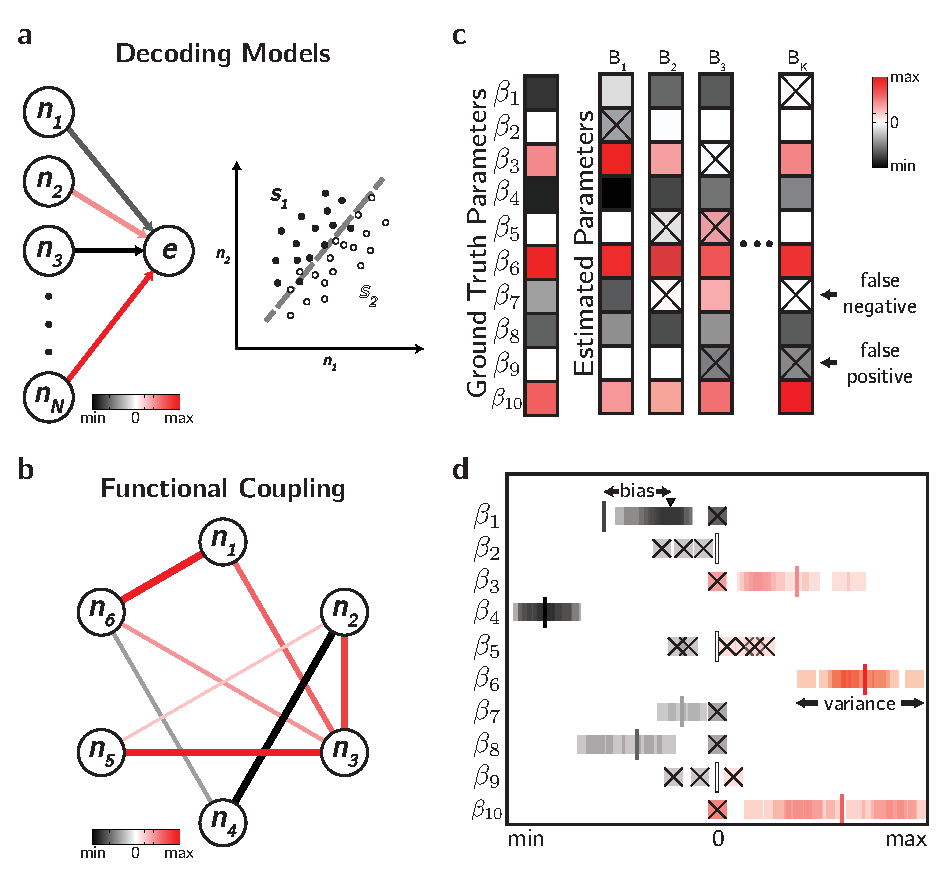
\includegraphics{./img/Fig1/Fig1}}
\end{figure}

\begin{figure}[b]
    \centering
    \scalebox{0.50}{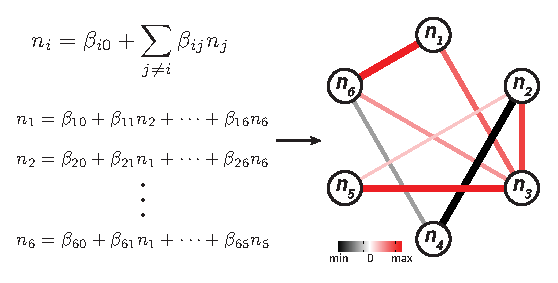
\includegraphics{./img/Fig2/Fig2}}
\end{figure}

\begin{figure}[b]
    \centering
    \scalebox{0.50}{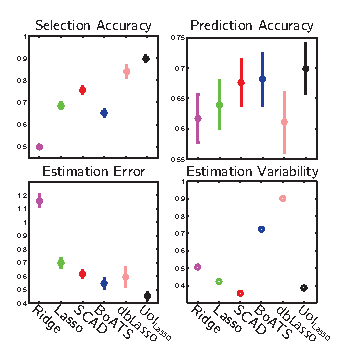
\includegraphics{./img/Fig3/Fig3}}
\end{figure}

\begin{figure}[b]
    \centering
    \scalebox{0.50}{\includegraphics{./img/Fig4/Fig4}}
\end{figure}
\section{CONCLUSIONS}


\addtolength{\textheight}{-12cm}   % This command serves to balance the column lengths
                                  % on the last page of the document manually. It shortens
                                  % the textheight of the last page by a suitable amount.
                                  % This command does not take effect until the next page
                                  % so it should come on the page before the last. Make
                                  % sure that you do not shorten the textheight too much.

%%%%%%%%%%%%%%%%%%%%%%%%%%%%%%%%%%%%%%%%%%%%%%%%%%%%%%%%%%%%%%%%%%%%%%%%%%%%%%%%



%%%%%%%%%%%%%%%%%%%%%%%%%%%%%%%%%%%%%%%%%%%%%%%%%%%%%%%%%%%%%%%%%%%%%%%%%%%%%%%%



%%%%%%%%%%%%%%%%%%%%%%%%%%%%%%%%%%%%%%%%%%%%%%%%%%%%%%%%%%%%%%%%%%%%%%%%%%%%%%%%

\section*{ACKNOWLEDGMENT}

P.S. Sachdeva was supported by the Department of Defense (DoD) through the National Defense Science \& Engineering Graduate Fellowship (NDSEG) Program.


%%%%%%%%%%%%%%%%%%%%%%%%%%%%%%%%%%%%%%%%%%%%%%%%%%%%%%%%%%%%%%%%%%%%%%%%%%%%%%%%

References are important to the reader; therefore, each citation must be complete and correct. If at all possible, references should be commonly available publications.



\begin{thebibliography}{99}

\bibitem{c1} G. O. Young, Synthetic structure of industrial plastics (Book style with paper title and editor), in Plastics, 2nd ed. vol. 3, J. Peters, Ed.  New York: McGraw-Hill, 1964, pp. 15�64.
\bibitem{c2} W.-K. Chen, Linear Networks and Systems (Book style).	Belmont, CA: Wadsworth, 1993, pp. 123�135.
\bibitem{c3} H. Poor, An Introduction to Signal Detection and Estimation.   New York: Springer-Verlag, 1985, ch. 4.
\bibitem{c4} B. Smith, �An approach to graphs of linear forms (Unpublished work style),� unpublished.
\bibitem{c5} E. H. Miller, �A note on reflector arrays (Periodical style�Accepted for publication),� IEEE Trans. Antennas Propagat., to be publised.
\bibitem{c6} J. Wang, �Fundamentals of erbium-doped fiber amplifiers arrays (Periodical style�Submitted for publication),� IEEE J. Quantum Electron., submitted for publication.
\bibitem{c7} C. J. Kaufman, Rocky Mountain Research Lab., Boulder, CO, private communication, May 1995.
\bibitem{c8} Y. Yorozu, M. Hirano, K. Oka, and Y. Tagawa, �Electron spectroscopy studies on magneto-optical media and plastic substrate interfaces(Translation Journals style),� IEEE Transl. J. Magn.Jpn., vol. 2, Aug. 1987, pp. 740�741 [Dig. 9th Annu. Conf. Magnetics Japan, 1982, p. 301].
\bibitem{c9} M. Young, The Techincal Writers Handbook.  Mill Valley, CA: University Science, 1989.
\bibitem{c10} J. U. Duncombe, �Infrared navigation�Part I: An assessment of feasibility (Periodical style),� IEEE Trans. Electron Devices, vol. ED-11, pp. 34�39, Jan. 1959.
\bibitem{c11} S. Chen, B. Mulgrew, and P. M. Grant, �A clustering technique for digital communications channel equalization using radial basis function networks,� IEEE Trans. Neural Networks, vol. 4, pp. 570�578, July 1993.
\bibitem{c12} R. W. Lucky, �Automatic equalization for digital communication,� Bell Syst. Tech. J., vol. 44, no. 4, pp. 547�588, Apr. 1965.
\bibitem{c13} S. P. Bingulac, �On the compatibility of adaptive controllers (Published Conference Proceedings style),� in Proc. 4th Annu. Allerton Conf. Circuits and Systems Theory, New York, 1994, pp. 8�16.
\bibitem{c14} G. R. Faulhaber, �Design of service systems with priority reservation,� in Conf. Rec. 1995 IEEE Int. Conf. Communications, pp. 3�8.
\bibitem{c15} W. D. Doyle, �Magnetization reversal in films with biaxial anisotropy,� in 1987 Proc. INTERMAG Conf., pp. 2.2-1�2.2-6.
\bibitem{c16} G. W. Juette and L. E. Zeffanella, �Radio noise currents n short sections on bundle conductors (Presented Conference Paper style),� presented at the IEEE Summer power Meeting, Dallas, TX, June 22�27, 1990, Paper 90 SM 690-0 PWRS.
\bibitem{c17} J. G. Kreifeldt, �An analysis of surface-detected EMG as an amplitude-modulated noise,� presented at the 1989 Int. Conf. Medicine and Biological Engineering, Chicago, IL.
\bibitem{c18} J. Williams, �Narrow-band analyzer (Thesis or Dissertation style),� Ph.D. dissertation, Dept. Elect. Eng., Harvard Univ., Cambridge, MA, 1993. 
\bibitem{c19} N. Kawasaki, �Parametric study of thermal and chemical nonequilibrium nozzle flow,� M.S. thesis, Dept. Electron. Eng., Osaka Univ., Osaka, Japan, 1993.
\bibitem{c20} J. P. Wilkinson, �Nonlinear resonant circuit devices (Patent style),� U.S. Patent 3 624 12, July 16, 1990. 






\end{thebibliography}




\end{document}
